\section{Allgemeine Krankheitslehre}

\subsection{Lehrinhalte "klinische Medizin"}
	\begin{itemize}
		\item \textbf{allgemeine Grundlagen der Krankheitslehre}
		\item \textbf{häufige Erkrankungen im Detail}
		\item \textbf{Diagnostik}
		\item \textbf{Therapie}
	\end{itemize}

\subsection{allgemeine Pathologie}
	\begin{itemize}
		\item \textbf{Definition}
			\begin{itemize}
				\item \textbf{Pathos, Logos}
				\item \textbf{Lehre von den Krankheiten (ihren Ursachen und den  Veränderungen, die sie im Organismus hervorrufen)}
			\end{itemize}
		\item \textbf{Ätiologie}
			\begin{itemize}
				\item \textbf{Lehre von den Krankheitsursachen}
			\end{itemize}
		\item \textbf{Pathogenese}
			\begin{itemize}
				\item \textbf{Lehre von der Entstehung einer Krankheit}
			\end{itemize}
	\end{itemize}

\subsection{Epidemiologie}
	\begin{itemize}
		\item \textbf{ursprüngliche Bedeutung: "Seuchenkunde"}
		\item \textbf{WHO Definition}
			\begin{itemize}
				\item \textbf{die Epidemiologie befasst sich mit der Untersuchung der Verteilung von Krankheiten, physiologischen Variablen und sozialen Krankheitsfolgen in menschlichen Bevölkerungsgruppen sowie mit Faktoren, die diese Verteilung beeinflussen}
				\item \textbf{Begriffsdefinitionen}
					\begin{itemize}
						\item \textbf{Gesundheit, Krankheit}
						\item \textbf{Morbidität, Mortalität, Letalität}
						\item \textbf{Inzidenz, Prävalenz}
					\end{itemize}
		\end{itemize}
	\end{itemize}

\subsection{Epidemiologie}
	\begin{itemize}
		\item \textbf{Gesundheit}
			\begin{itemize}
				\item \textbf{Zustand völligen körperlichen, seelischen und sozialen Wohlbefindens}
			\end{itemize}
		\item \textbf{Krankheit}
			\begin{itemize}
				\item \textbf{Störung in diesem körperlich-seelisch-geistig-sozialen Gleichgewicht}
			\end{itemize}
		\item \textbf{Morbidität}
			\begin{itemize}
				\item \textbf{Häufigkeit einer bestimmten Krankheit in einer Bevölkerungsgruppe}
				\item \textbf{Verhältnis der Zahl der Erkrankungen zur Zahl der Gesamtbevölkerung in einem bestimmten Zeitraum}
			\end{itemize}
		\item \textbf{Mortalität ("Sterblichkeit")}
			\begin{itemize}
				\item \textbf{Häufigkeit einer bestimmten Kh als Todesursache in einer Bevölkerungsgruppe}
				\item \textbf{Verhältnis der Zahl der Todesfälle an bestimmter Erkrankung zur Zahl der Gesamtbevölkerung in einem bestimmten Zeitraum, i.d.R. 1 Jahr, pro 100000 Einwohner}
			\end{itemize}
	\pagebreak
		\item \textbf{Letalität ("Tödlichkeit")}
			\begin{itemize}
				\item \textbf{Zahl der Todesfälle bezogen auf die Zahl der Erkrankten}
				\item \textbf{Verhältnis der Zahl der Todesfälle zur Zahl der an einer bestimmten Krankheit Erkrankten ("Mortalität in \%")}
			\end{itemize}
		\item \textbf{Inzidenz (= Erkrankungshäufigkeit)}
			\begin{itemize}
				\item \textbf{Zahl von Neuerkrankungen an einer bestimmten KH innerhalb eines bestimmten Zeitraumes}
				\item \textbf{Anzahl der Personen, die im Verlauf eines bestimmten Zeitraumes (i.d.R. 1 Jahr) an einer bestimmten Krankheit erstmals erkranken}
			\end{itemize}
		\item \textbf{Prävalenz}
			\begin{itemize}
				\item \textbf{Zahl der zu einem bestimmten Zeitpunkt an einer bestimmten KH leidenden Personen, bezogen auf die Gesamtbevölkerung}
			\end{itemize}
	\end{itemize}

\subsection{Methoden der pathologischen Diagnostik}
	\begin{itemize}
		\item \textbf{intravitale Diagnostik}
			\begin{itemize}
				\item \textbf{zytologische Untersuchungsmethoden}
				\item \textbf{histologische Untersuchungsmethoden}
			\end{itemize}
		\item \textbf{postmortale Diagnostik}
			\begin{itemize}
				\item \textbf{sanitätspolizeiliche Obduktion}
				\item \textbf{gerichtsmedizinische Obduktion}
				\item \textbf{klinische Obduktion}
			\end{itemize}
	\end{itemize}

\subsection{intravitale Diagnostik}
	\begin{itemize}
		\item \textbf{zytologische Untersuchungsmethoden}
			\begin{itemize}
				\item \textbf{Analyse von Einzelzellen}
				\item \textbf{Gewinnung der Zellen}
					\begin{itemize}
						\item \textbf{von Schleimhautoberflächen, Sekreten, Spülflüssigkeiten}
						\item \textbf{durch Punktion von Flüssigkeiten}
						\item \textbf{durch Feinnadelpunktion von Organen}
					\end{itemize}
				\item \textbf{Zweck / häufige Fragestellungen}
					\begin{itemize}
						\item \textbf{infektiöse Erkrankungen (Erregernachweis) und deren Folgen}
						\item \textbf{Entzündungsdiagnostik}
						\item \textbf{Tumorzellnachweis, etc.}
					\end{itemize}
			\end{itemize}
		\item \textbf{histologische Untersuchungsmethoden}
			\begin{itemize}
				\item \textbf{Analyse von Gewebeschnitten von chirurgisch oder bioptisch gewonnenen Gewebestücken}
				\item \textbf{Gefrierschnellschnitt, Paraffinschnitt}
				\item \textbf{Analysetechniken}
					\begin{itemize}
						\item \textbf{Lichtmikroskopi}
							\begin{itemize}
								\item \textbf{Anfertigung von Paraffinschnitten oder Gefrierschnitten}
							\end{itemize}
						\item \textbf{Immunfluoreszenz}
						\item \textbf{Elektronenmikroskopie}
					\end{itemize}
		\item \textbf{Zweck / häufige Fragestellungen}
			\begin{itemize}
				\item \textbf{Zellbeurteilung im Gewebeverband, Tumordiagnostik, Kontrolle des chirurgischen Eingriffs (Resektionsränder), etc.}
			\end{itemize}
		\end{itemize}
	\end{itemize}
	
\begin{center}
	\includegraphics[scale=0.5]{{klin.med.-grundlagen-img0000}.png}
\end{center}

\subsection{intravitale Diagnostik}
	\begin{itemize}
		\item \textbf{bakteriologische und serologische Diagnostik}
			\begin{itemize}
				\item \textbf{mikroskopischer Nachweis von Krankheitserregern}
					\begin{itemize}
						\item \textbf{spezielle Färbemethoden zur Darstellung der Mikroorganismen}
							\begin{itemize}
								\item \textbf{Lichtmikroskopie}
								\item \textbf{Elektronenmikroskopie}
							\end{itemize}
					\end{itemize}
				\item \textbf{kultureller Nachweis von Krankheitserregern}
					\begin{itemize}
						\item \textbf{Bakterienkultur auf flüssigen oder festen Nährmedien}
					\end{itemize}
				\item \textbf{serologischer Nachweis von Krankheitserregern}
					\begin{itemize}
						\item \textbf{Antigen-Antikörper-Reaktion}
						\item \textbf{Agglutinationsreaktionen}
							\begin{itemize}
								\item \textbf{Antigen-Suchtest}
								\item \textbf{Antikörper-Suchtest}
							\end{itemize}
					\end{itemize}
			\end{itemize}
		\item \textbf{Spezialmethoden}
			\begin{itemize}
				\item \textbf{Elektronenmikroskopie}
				\item \textbf{Immunhistochemie}
					\begin{itemize}
						\item \textbf{Sichtbarmachen spezieller Zell- und Gewebe-Strukturen durch spezifische AG-AK-Reaktionen mittels monoklonaler AK}
					\end{itemize}
				\item \textbf{biochemische Untersuchungen}
					\begin{itemize}
						\item \textbf{Nachweis bestimmter Strukturen aus Körperflüssigkeiten}
						\item \textbf{Techniken: Immuno-Assay, Blotting-Verfahren (Immunoblot)}
					\end{itemize}
				\item \textbf{molekularbiologische Techniken}
					\begin{itemize}
						\item \textbf{Hybridisierungsmethoden}
						\item \textbf{Amplifizierungsmethoden}
					\end{itemize}
		\end{itemize}
	\end{itemize}

\pagebreak
\subsection{postmortale Diagnostik}
	\begin{itemize}
		\item \textbf{Obduktion, Sektion, innere Leichenbeschau, Autopsie}
			\begin{itemize}
				\item \textbf{sanitätspolizeiliche Obduktion}
					\begin{itemize}
						\item \textbf{bei ungenügender Information}
					\end{itemize}
				\item \textbf{gerichtsmedizinische Obduktion}
					\begin{itemize}
						\item \textbf{bei Verdacht auf Fremdverschulden}
					\end{itemize}
				\item \textbf{klinische Obduktion}
					\begin{itemize}
						\item \textbf{zur Qualitätskontrolle}
					\end{itemize}
				\item \textbf{Zweck}
					\begin{itemize}
						\item \textbf{Grundlage für Statistiken und gesundheitspolitische Maßnahmen}
						\item \textbf{wissenschaftliche Aufgaben}
						\item \textbf{rechtliche Grundlagen siehe Krankenanstaltengesetz}
					\end{itemize}
			\end{itemize}
	\end{itemize}

\subsection{Übersicht: Krankheitsursachen, -Verlauf, -Ausgang}
	\begin{itemize}
		\item \textbf{Krankheitsursachen (Ätiologie)}
			\begin{itemize}
				\item \textbf{endogene Krankheitsursachen}
				\item \textbf{exogene Krankheitsursachen}
			\end{itemize}
		\item \textbf{Krankheitsverlauf}
			\begin{itemize}
				\item \textbf{nach zeitlichem Verlauf}
				\item \textbf{Rezidiv, Remission}
			\end{itemize}
		\item \textbf{Krankheitsausgang}
	\end{itemize}

\subsection{Krankheitsursachen}
	\begin{itemize}
		\item \textbf{innere (endogene) Krankheitsursachen}
			\begin{itemize}
				\item \textbf{genetische Störungen}
					\begin{itemize}
						\item \textbf{Chromosomenschäden, DNA-Schäden}
					\end{itemize}
				\item \textbf{Disposition}
					\begin{itemize}
						\item \textbf{Altersdisposition, Geschlechtsdisposition, genetische Disposition, patholog. Disposition}
					\end{itemize}
				\item \textbf{Autoimmunerkrankungen}
				\item \textbf{hormonelle (endokrine) Störungen}
			\end{itemize}
		\item \textbf{äußere (exogene) Krankheitsursachen}
		\item \textbf{Noxen}
			\begin{itemize}
				\item \textbf{eine Noxe ist eine Substanz oder ein Ereignis, das einem biologischen Organismus Schäden zufügt}
				\item \textbf{im weiteren Sinn versteht man unter einer "Noxe" jede Art von äußerer Krankheitsursache}
			\end{itemize}
	\end{itemize}
\pagebreak
\subsection{Krankheitsursachen - Noxen}
	\begin{itemize}
		\item \textbf{physikalische Noxen}
			\begin{itemize}
				\item \textbf{mechanische Einwirkung}
					\begin{itemize}
						\item \textbf{akut: Trauma (Quetschung, Schnitt, Druck: Barotrauma, …..)}
						\item \textbf{chronisch: Dekubitus}
					\end{itemize}
				\item \textbf{thermische Einwirkung}
					\begin{itemize}
						\item \textbf{Verbrennungen, Erfrierungen}
					\end{itemize}
				\item \textbf{Luftdruckveränderungen}
					\begin{itemize}
						\item \textbf{Höhenkrankheit, Dekompressionssyndrom}
					\end{itemize}
				\item \textbf{Stromeinwirkung}
					\begin{itemize}
						\item \textbf{Verbrennung, Herzrhythmusstörung, Atemlähmung}
					\end{itemize}
				\item \textbf{Strahleneinwirkung}
					\begin{itemize}
						\item \textbf{UV-Strahlen, ionisierende Strahlung}
					\end{itemize}
			\end{itemize}
		\item \textbf{biologische Noxen}
			\begin{itemize}
				\item \textbf{lebende Krankheitserreger: Bakterien, Viren, Pilze, Würmer, $\dots$}
				\item \textbf{Toxine von Bakterien, Pilzen, Pflanzen, Tieren}
			\end{itemize}
		\item \textbf{chemisch-toxische Noxen}
			\begin{itemize}
				\item \textbf{Laugen oder Säuren}
				\item \textbf{anorganische Verbindungen: Metalle, Staube, Gase}
				\item \textbf{organische Verbindungen: Alkohol, aromatische Amine, $\dots$}
			\end{itemize}
		\item \textbf{fehlerhafte Nahrungszufuhr und/oder – Verwertung}
			\begin{itemize}
				\item \textbf{Menge, Zusammensetzung, Aufnahme, $\dots$}
			\end{itemize}
		\item \textbf{psychosoziale Faktoren (Noxe = ?)}
	\end{itemize}

\subsection{Krankheitsverlauf}
	\begin{itemize}
		\item \textbf{perakut}
			\begin{itemize}
				\item \textbf{besonders rasch, heftig, oft lebensbedrohlich}
				\item \textbf{foudroyant (oder: fulminant) = "blitzartig" einsetzend und verlaufend}
			\end{itemize}
		\item \textbf{akut}
			\begin{itemize}
				\item \textbf{plötzlicher Beginn, ausgeprägte Symptome (z.B. Lungenembolie)}
			\end{itemize}
		\item \textbf{subakut}
			\begin{itemize}
				\item \textbf{allmählicher Beginn (z.B. Hepatitis B)}
			\end{itemize}
		\item \textbf{chronisch}
			\begin{itemize}
				\item \textbf{schleichender, längerer Verlauf, Symptome weniger ausgeprägt (z.B. MS)}
			\end{itemize}
		\item \textbf{rezidivierend}
			\begin{itemize}
				\item \textbf{wiederkehrend}
			\end{itemize}
		\item \textbf{Rezidiv}
			\begin{itemize}
				\item \textbf{Wiederauftreten der selben KH nach völliger Abheilung oder nach symptomfreiem Intervall}
			\end{itemize}
		\item \textbf{Remission}
			\begin{itemize}
				\item \textbf{Zeitspanne der klinischen Symptomfreiheit einer in Schüben verlaufenden Erkrankung}
			\end{itemize}
	\end{itemize}

\subsection{Krankheitsausgang}
	\begin{itemize}
		\item \textbf{Heilung}
			\begin{itemize}
				\item \textbf{Restitutio ad integrum = völlige Wiederherstellung}
			\end{itemize}
		\item \textbf{Defektheilung}
			\begin{itemize}
				\item \textbf{Reparatio = bleibender Defekt}
				\item \textbf{z.B. Ersatz durch minderwertiges Narbengewebe}
			\end{itemize}
		\item \textbf{Tod}
			\begin{itemize}
				\item \textbf{die genaue Grenze zwischen Leben und Tod ist schwer zu definieren}
				\item \textbf{so können Patienten mit Herzstillstand manchmal erfolgreich wiederbelebt werden}
				\item \textbf{einzelne Zellen und Gewebe können noch viele Stunden nach eingetretenem Hirntod auf äußere Einflüsse reagieren}
			\end{itemize}
	\end{itemize}

\subsection{Tod}
	\begin{itemize}
		\item \textbf{klinischer Tod}
			\begin{itemize}
				\item \textbf{völliger Kreislaufstillstand; durch Reanimation aufhebbar, solange Funktion des ZNS noch erhalten (Wiederbelebungszeit)}
				\item \textbf{unsichere Todeszeichen}
			\end{itemize}
		\item \textbf{biologischer Tod}
			\begin{itemize}
				\item \textbf{Aufhören aller Organ- und Zellfunktionen}
				\item \textbf{sichere Todeszeichen}
			\end{itemize}
		\item \textbf{Hirntod}
			\begin{itemize}
				\item \textbf{irreversibler Ausfall aller Hirnfunktionen  $\rightarrow$  Transplantationschirurgie}
				\item \textbf{objektive Feststellung: Nulllinien-EEG etc.}
			\end{itemize}
	\end{itemize}

\subsection{Todeszeichen}
	\begin{itemize}
		\item \textbf{unsichere Todeszeichen}
			\begin{itemize}
				\item \textbf{Blässe der Haut und Abkühlung}
				\item \textbf{Aufhören der Atemfunktion und der Herz-Kreislauf-Funktion}
					\begin{itemize}
						\item \textbf{fehlende Atmung}
						\item \textbf{fehlender Puls}
						\item \textbf{fehlender Herzschlag}
					\end{itemize}
				\item \textbf{Aufhören der ZNS-Funktion}
					\begin{itemize}
						\item \textbf{Bewusstlosigkeit}
						\item \textbf{fehlender Pupillenreflex (vgl. Areflexie)}
						\item \textbf{komplette Lähmung aller Muskeln}
					\end{itemize}
			\end{itemize}
		\item \textbf{sichere Todeszeichen}
			\begin{itemize}
				\item \textbf{Verletzungen, die mit dem Leben nicht mehr vereinbar sind (z.B. Fehlen des Kopfes)}
				\item \textbf{Totenkälte (Algor mortis)}
				\item \textbf{Totenflecken (Livores)}
				\item \textbf{Totenstarre (Rigor mortis, Leichenstarre)}
				\item \textbf{Autolyse (Verwesung) und Fäulnis}
			\end{itemize}
	\end{itemize}

\section{Zellschäden - gewebeschäden}

\subsection{Übersicht}
	\begin{itemize}
		\item \textbf{Regeneration – Reparation}
		\item \textbf{Zellschäden}
			\begin{itemize}
				\item \textbf{Ursachen}
				\item \textbf{reversible Zellschäden}
					\begin{itemize}
						\item \textbf{Dystrophie}
					\end{itemize}
				\item \textbf{irreversible Zellschäden}
					\begin{itemize}
						\item \textbf{Apoptose}
						\item \textbf{Nekrose}
					\end{itemize}
				\item \textbf{Zellwachstumsstörungen}
					\begin{itemize}
						\item \textbf{quantitative Zellwachstumsstörungen}
						\item \textbf{qualitative Zellwachstumsstörungen}
					\end{itemize}
			\end{itemize}
	\end{itemize}

\subsection{Regeneration - Reparation}
	\begin{itemize}
		\item \textbf{Ersatz von verlorengegangenen Zellen oder Geweben durch Zell- und Gewebsneubildung}
		\item \textbf{physiologische Regeneration}
			\begin{itemize}
				\item \textbf{Zellersatz von durch natürlichen Verschleiß verlorengegangenen Zellen}
				\item \textbf{die ursprüngliche Struktur und Funktion bleibt erhalten}
			\end{itemize}
		\item \textbf{pathologischer Gewebeersatz}
			\begin{itemize}
				\item \textbf{Ersatz von Geweben, die durch krankhafte Einflüsse zugrunde gegangen sind}
					\begin{itemize}
						\item \textbf{vollständige pathologische \emph{Regeneration}: Ersatz defekter Zellen und Gewebe durch morphologisch gleichartige und funktionell gleichwertige Strukturen}
						\item \textbf{\emph{Reparation}: Ersatz durch Ersatzgewebsbildung (Defektheilung)}
					\end{itemize}
			\end{itemize}
		\item \textbf{proliferatives Potential von Geweben und Zellen}
			\begin{itemize}
				\item \textbf{Wechselgewebe = labiles Gewebe}
					\begin{itemize}
						\item \textbf{Häute/Schleimhäute (Epithel)}
						\item \textbf{Knochenmark}
					\end{itemize}
				\item \textbf{ruhendes = stabiles Gewebe}
					\begin{itemize}
						\item \textbf{Parenchymzellen, z.B. Leber, Pankreas}
						\item \textbf{Mesenchymzellen, z.B. Fibroblasten, glatte Muskelzellen, Chondrozyten, Osteozyten, Endothelien}
					\end{itemize}
				\item \textbf{permanentes Gewebe}
					\begin{itemize}
						\item \textbf{Neurone}
						\item \textbf{Skelettmuskulatur}
						\item \textbf{Herzmuskel}
					\end{itemize}
			\end{itemize}
	\end{itemize}
\pagebreak
\subsection{Ursachen des Zellschadens (Noxen)}
	\begin{itemize}
		\item \textbf{Hypoxie ( $\rightarrow$  hypoxische Zellschädigung)}
			\begin{itemize}
				\item \textbf{häufigster Mechanismus einer Zellschädigung}
				\item \textbf{Mangeldurchblutung durch Hypotonie, Arteriosklerose, Thrombose, $\dots$}
			\end{itemize}
		\item \textbf{chemische Substanzen}
			\begin{itemize}
				\item \textbf{toxische Wirkung konzentrationsabhängig, sehr breites Spektrum potentieller Noxen und Angriffspunkte an der Zelle}
			\end{itemize}
		\item \textbf{Infektion}
			\begin{itemize}
				\item \textbf{Viren, Bakterien, Pilze, Parasiten mit sehr verschiedenen meist gut definierten zellulären Schädigungsmechanismen (DNA-Schädigung, Toxinwirkung, Immunreaktion)}
			\end{itemize}
		\item \textbf{Immunreaktionen}
			\begin{itemize}
				\item \textbf{Erregerabwehr (v.a. virale Infektionen), Autoimmunerkrankungen, Transplantatabstoßung}
			\end{itemize}
		\item \textbf{genetische Defekte}
			\begin{itemize}
				\item \textbf{führen zu komplexen Multiorganstörungen (z.B. Trisomien)  oder pathogenen Veränderungen einzelner Proteine durch Punktmutationen (z.B. Sichelzellanämie)}
			\end{itemize}
		\item \textbf{inadäquate Ernährung}
			\begin{itemize}
				\item \textbf{klassischerweise Mangelernährung (z.B. Vitamine)}
				\item \textbf{in Industrienationen aber auch Überangebot, vor allem an Lipiden und Kohlehydraten}
			\end{itemize}
		\item \textbf{physikalische Einwirkungen}
			\begin{itemize}
				\item \textbf{mechanische Traumen, Temperatur, Strom,  nichtionisierende (UV) und ionisierende (Röntgen, Radioaktivität) Strahlung}
			\end{itemize}
	\end{itemize}

\subsection{Zell- und Gewebereaktionen auf Noxen}
	\begin{itemize}
		\item \textbf{Zellschäden}
			\begin{itemize}
				\item \textbf{reversibel: "Dystrophie"}
				\item \textbf{irreversibel: Nekrose, Apoptose}
			\end{itemize}
		\item \textbf{quantitative Differenzierungsstörung (meist Anpassungsreaktion)}
			\begin{itemize}
				\item \textbf{Agenesie, Aplasie, Hypoplasie}
				\item \textbf{Atrophie}
				\item \textbf{Hypertrophie, Hyperplasie}
			\end{itemize}
		\item \textbf{qualitative Differenzierungsstörung}
			\begin{itemize}
				\item \textbf{Metaplasie}
				\item \textbf{Dysplasie}
				\item \textbf{Anaplasie}
			\end{itemize}
	\end{itemize}

\subsection{reversible Zellschädigungen}
	\begin{itemize}
		\item \textbf{reversible Zellschädigungen  $\rightarrow$  "point of no return"  $\rightarrow$  irreversible Zellschädigung (Zelltod)}
		\item \textbf{Quantität der Noxe entscheidend}
		\item \textbf{reversible Zellschädigungen: "Dystrophien"}
			\begin{itemize}
				\item \textbf{Zellödem ("trübe Schwellung")}
				\item \textbf{intrazelluläre Verfettung (fettige Dystrophie)}
				\item \textbf{hyaline Dystrophie / Degeneration}
			\end{itemize}
	\end{itemize}

\subsection{irreversible Zellschädigungen}
	\begin{itemize}
		\item \textbf{irreversible Zellschädigungen}
			\begin{itemize}
				\item \textbf{Apoptose}
				\item \textbf{Nekrose}
					\begin{itemize}
						\item \textbf{Kennzeichen der Nekrose}
						\item \textbf{Nekroseformen}
						\item \textbf{Folgen der Nekrose}
					\end{itemize}
			\end{itemize}
	\end{itemize}

\subsection{Apoptose}
	\begin{itemize}
		\item \textbf{Apoptose = programmierter Zelltod}
			\begin{itemize}
				\item \textbf{genetisch fixiertes "Selbstmordprogramm" einer Zelle}
				\item \textbf{Programm zur Elimination einzelner Zellen deren Funktion nicht mehr benötigt wird oder die einen irreparablen (genetischen) Schaden erlitten haben}
				\item \textbf{kann von außen angeregt (extrinisisch) oder durch  zellinterne Mechanismen (intrinsisch) initiiert werden}
				\item \textbf{aktiver streng gesteuerter Prozess durch den sichergestellt wird, dass die betroffene Zelle ohne Schädigung des Nachbargewebes zugrundegeht}
				\item \textbf{typische Veränderungen}
					\begin{itemize}
						\item \textbf{Kernschrumpfung, Zellorganellen und Zellkontakte lösen sich auf}
					\end{itemize}
			\end{itemize}
		\item \textbf{Apoptose als genetisch programmiertes, geregeltes Absterben von Zellen (physiologische Form des Zelltodes)}
			\begin{itemize}
				\item \textbf{während der Embryonalentwicklung}
				\item \textbf{während des Lebens und Alterns}
			\end{itemize}
		\item \textbf{Apoptose als induziertes Absterben der Zellen}
			\begin{itemize}
				\item \textbf{Effekt eines Virusbefalls, einer Immunreaktion oder von Zytokinen, $\dots$}
			\end{itemize}
	\end{itemize}

\subsection{Nekrose}
	\begin{itemize}
		\item \textbf{Nekrose = provozierter Zelltod}
			\begin{itemize}
				\item \textbf{Endstrecke einer irreversiblen Stoffwechselstörung}
				\item \textbf{passiver Prozess, die Zelle versucht jedoch zuerst durch eine Anpassungsreaktion der Schädigung zu entgehen}
				\item \textbf{typische Veränderungen}
					\begin{itemize}
						\item \textbf{Zytoplasmaveränderungen (Eosinophilie des Plasmas)}
						\item \textbf{Zellkernveränderungen (Karyolyse $\rightarrow$ Diagnostik!)}
						\item \textbf{Zerstörung der Zellmembran mit Übertritt von intrazellulären Enzymen in die Umgebung und ins Blut}
						\item \textbf{Reaktion des umgebenden Gewebes}
							\begin{itemize}
								\item \textbf{hyperämischer Randsaum}
								\item \textbf{leukozytärer Demarkationswall}
								\item \textbf{Granulationsgewebe}
							\end{itemize}
					\end{itemize}
			\end{itemize}
		\item \textbf{Nekroseformen}
			\begin{itemize}
				\item \textbf{Koagulationsnekrose}
				\item \textbf{Kolliquationsnekrose}
				\item \textbf{käsige Nekrose}
				\item \textbf{gangränöse Nekrose}
				\item \textbf{hämorrhagische Nekrose}
			\end{itemize}
		\item \textbf{Folgen der Nekrose}
			\begin{itemize}
				\item \textbf{restitutio ad integrum}
				\item \textbf{Defektheilung / Narbenbildung}
				\item \textbf{Hohlraumbildung (Zyste etc.)}
				\item \textbf{Ulkusbildung}
			\end{itemize}
	\end{itemize}

\subsection{Übersicht: Zellwachstumsstörungen}
	\begin{itemize}
		\item \textbf{pathologisches Zellwachstum}
			\begin{itemize}
				\item \textbf{quantitative Wachstumsstörungen}
					\begin{itemize}
						\item \textbf{Verminderung des Zellwachstums = Atrophie}
						\item \textbf{angeborene Störungen mit Hemmung des Wachstums}
						\item \textbf{Vermehrung des Zellwachstums = Hypertrophie, Hyperplasie}
					\end{itemize}
				\item \textbf{qualitative Zellwachstumsstörungen}
					\begin{itemize}
						\item \textbf{Metaplasie, Dysplasie, Anaplasie}
					\end{itemize}
			\end{itemize}
	\end{itemize}

\subsection{Anpassungsreaktionen auf zellulären Stress}
	\begin{center}
		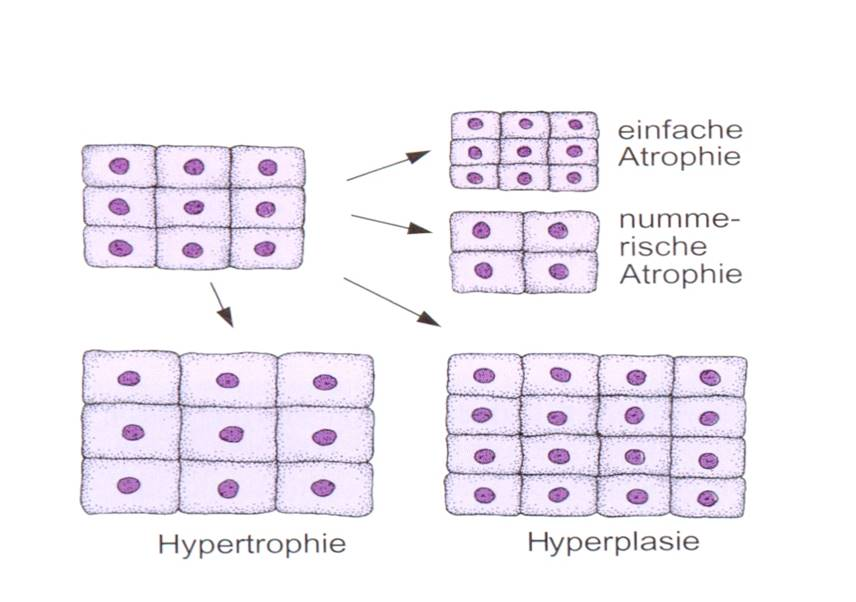
\includegraphics[scale=0.5]{Picture1.jpg}
	\end{center}

\subsection{quantitative Wachstumsstörungen}
	\begin{itemize}
		\item \textbf{Atrophie = Verminderung des Zellwachstums}
			\begin{itemize}
				\item \textbf{Verkleinerung eines primär normal entwickelten und normal großen Gewebes bzw. Organs}
				\item \textbf{Überwiegen der katabolen über die anabolen Stoffwechselvorgänge}
					\begin{itemize}
						\item \textbf{einfache Atrophie: Zellverkleinerung}
						\item \textbf{numerische Atrophie: Verminderung der Zellzahl}
					\end{itemize}
				\item \textbf{physiologische Atrophie}
					\begin{itemize}
						\item \textbf{im Rahmen normaler physiologischer Entwicklungsprozesse}
					\end{itemize}
				\item \textbf{pathologische Atrophie}
					\begin{itemize}
						\item \textbf{im Rahmen krankhafter Ereignisse, Überwiegen der katabolen Prozesse}
					\end{itemize}
			\end{itemize}
	\end{itemize}
\pagebreak
\subsection{quantitative Wachstumsstörungen}
	\begin{itemize}
		\item \textbf{lokale Atrophien}
			\begin{itemize}
				\item \textbf{auf ein Organ oder einen Gewebsabschnitt beschränkt}
					\begin{itemize}
						\item \textbf{Inaktivitätsatrophie}
						\item \textbf{vaskuläre Atrophie $\rightarrow$ Ischämie}
						\item \textbf{mechanische Druckatrophie $\rightarrow$ Kompression}
						\item \textbf{neurogene Atrophie (fehlende Innervation)}
						\item \textbf{Erschöpfungsatrophie}
						\item \textbf{endokrine Atrophie (mangelnder hormoneller Stimulus)}
						\item \textbf{genetisch bedingte Atrophie}
					\end{itemize}
				\item \textbf{generalisierte Atrophien}
					\begin{itemize}
						\item \textbf{den gesamten Körper betreffend}
							\begin{itemize}
								\item \textbf{senile Atrophie}
								\item \textbf{Hungeratrophie}
								\item \textbf{Kachexie}
							\end{itemize}
				\end{itemize}
		\end{itemize}
		\item \textbf{angeborene Störungen mit Hemmung des Wachstums}
			\begin{itemize}
				\item \textbf{Agenesie: gesamte Organanlage fehlt}
				\item \textbf{Aplasie: Organentwicklung fand nicht statt}
				\item \textbf{Hypoplasie: Organentwicklung kam vorzeitig zum Stillstand (Unterentwicklung)}
			\end{itemize}
		\item \textbf{Hypertrophie}
			\begin{itemize}
				\item \textbf{Organvergrößerung durch Zellvergrößerung ohne Zellvermehrung}
				\item \textbf{Steigerung der Leistungsfähigkeit, jedoch Verminderung der Reserve}
					\begin{itemize}
						\item \textbf{Arbeitshypertrophie (vermehrte Arbeitsbelastung)}
						\item \textbf{kompensatorische Hypertrophie}
					\end{itemize}
			\end{itemize}
		\item \textbf{Hyperplasie}
			\begin{itemize}
				\item \textbf{Organvergrößerung durch Zellvermehrung}
				\item \textbf{regeneratorische Hyperplasie}
					\begin{itemize}
						\item \textbf{Reaktion auf Gewebeschädigung mit überschießender Regeneration / Reparation}
					\end{itemize}
				\item \textbf{Hyperplasien infolge endokriner Störungen}
					\begin{itemize}
						\item \textbf{vermehrter Hormonstimulus}
						\item \textbf{z.B. Hyperplasie der Prostata, Hyperplasie der Schilddrüse}
					\end{itemize}
			\end{itemize}
	\end{itemize}

\subsection{qualitative Wachstumsstörungen}
	\begin{itemize}
		\item \textbf{Metaplasie}
			\begin{itemize}
				\item \textbf{Ersatz eines ausdifferenzierten Gewebes durch anderes hochdifferenziertes Gewebe}
			\end{itemize}
		\item \textbf{Dysplasie}
			\begin{itemize}
				\item \textbf{meist noch reversible Veränderungen von Zellen durch atypische Regeneration und Verlust der Differenzierung fließender Übergang zur (irreversiblen) Anaplasie}
			\end{itemize}
		\item \textbf{Anaplasie}
			\begin{itemize}
				\item \textbf{irreversible Entdifferenzierung der Zellen und Gewebe mit Verlust der geweblichen Struktur und der Formbesonderheiten der Zellen = Malignität}
			\end{itemize}
	\end{itemize}